\documentclass{article}

%\usepackage{corl_2020} % Use this for the initial submission.
\usepackage{amsmath, amssymb}
\usepackage{amsmath,algorithm,algcompatible, algpseudocode, multirow, graphicx, caption, subcaption, gensymb, hyperref}
\DeclareMathOperator*{\argmin}{argmin}
\graphicspath{{./imgs/}}
%\usepackage[final]{corl_2020} % Uncomment for the camera-ready ``final'' version.
\usepackage[preprint]{corl_2020} % Uncomment for pre-prints (e.g., arxiv); This is like ``final'', but will remove the CORL footnote.
\usepackage{bbm}

\newcommand*{\varfont}{\fontfamily{pcr}\selectfont}

\title{A Comparative Study of Asymptotically-Optimal Sampling-Based Path Planning Methods}

% The \author macro works with any number of authors. There are two
% commands used to separate the names and addresses of multiple
% authors: \And and \AND.
%
% Using \And between authors leaves it to LaTeX to determine where to
% break the lines. Using \AND forces a line break at that point. So,
% if LaTeX puts 3 of 4 authors names on the first line, and the last
% on the second line, try using \AND instead of \And before the third
% author name.

% NOTE: authors will be visible only in the camera-ready and preprint versions (i.e., when using the option 'final' or 'preprint'). 
% 	For the initial submission the authors will be anonymized.

\author{
  Jazib Ahmad \\
  Department of Computer Science \\
  University of Toronto \\
  \texttt{jazibahmad@cs.toronto.edu} \\
  %% examples of more authors
  \And
  Jimmy Woo \\
  Department of Computer Science \\
  University of Toronto \\
  \texttt{jimmywoo@cs.toronto.edu} \\
  \And
  Sumant Bagri \\
  Department of Computer Science \\
  University of Toronto \\
  \texttt{sbagri@cs.toronto.edu} \\
}


\begin{document}
\maketitle

%===============================================================================

\begin{abstract}
In this project, we perform a comparative study between three asymptotically-optimal sampling-based path planning algorithms: Fast-marching trees (FMT*), batch informed trees (BIT*), and neural rapidly random-exploring trees (NRRT*). Each algorithm is implemented separately, and their simulated performances in terms of execution time and path costs is evaluated in different map environments with varying complexities and structural construct. The performance with varying sample counts is observed, and a qualitative comparison of the optimal paths achieved from each algorithm for a subset of the environments is provided to demonstrate how the planners handle obstacles.

In general, we found that BIT* is able to outperform both FMT* and NRRT* in terms of finding the most optimal path. It is also able to converge quickly in most scenarios. FMT* stands out in terms of making the minimum number of collision checks during path-finding which would prove extremely beneficial in high-dimensional state-space. In theory, NRRT* should compute near-optimal paths at very low execution times, but this reported behaviour was unverified due to limitations in the implementation of the algorithm. The algorithm implementations as well as the evaluation data and the plots are available on GitHub.\footnote{\url{https://github.com/jimmywoo1/CSC2630_Project}}

\end{abstract}

% Two or three meaningful keywords should be added here
\keywords{Sampling-based planning, asymptotically optimal planning} 

%===============================================================================

\section{Introduction}
Path planning is a search problem where the goal is to find a sequence of actions that will lead to an obstacle-free optimal path from a start state to a target state. Grid-based heuristic search algorithms \cite{astar} have been proposed in the past that guarantee finding optimal paths that exists. However, these techniques do not scale well to higher dimensional problems as they require discretization of the state space. On the other hand, sampling-based path planning algorithms \cite{rrt*} can solve high-dimensional path planning problems more efficiently. However, these algorithms only converge to optimal paths asymptotically, and in practice may compute sub-optimal paths. Many attempts have been made to make improvements to sampling-based methods \cite{irrt}\cite{SBA*}\cite{RA*}, using techniques such as heuristic guided searches, or the reduction of the sampling space. In this project, we implement three sampling-based path planning algorithms, and compare their performances through simulations.

We can formulate the path planning problem by defining the state space and the cost function similar to \cite{rrt*}. Let $\mathcal{X} \in \mathbb{R}^d$, $\mathcal{X}_{free}$, and $\mathcal{X}_{obs}$ be the state space, free space, and the obstacle space respectively where $\mathcal{X}_{obs} \subset \mathcal{X}$ and $\mathcal{X}_{free}  = \mathcal{X} \setminus \mathcal{X}_{obs}$. Let $x_{init} \in \mathcal{X}_{free}$, $x_{goal} \in \mathcal{X}_{free}$ be the start and target states respectively. The goal of the path planning problem is to determine a path $\sigma$ : [0, 1] $\mapsto \mathcal{X}_{free}$ such that $\sigma(0) = x_{init}$, $\sigma(1) = \mathcal{G}(x_{goal})$, where the acceptable goal region is defined as $\mathcal{G}(x_{goal}) = \{x \, \in \, \mathcal{X} \, | \, x - x_{goal} < r\}$. Then we can define the path planning problem as minimizing the following cost function:
    \begin{align}
        & \sigma^* = \argmin_{\sigma \in \Sigma} c(\sigma) \\
        & s.t. \;\, \sigma(0) = x_{init}, \; \sigma(1) = \mathcal{G}(x_{goal}), \; \sigma(t) \;  \mathcal{X}_{free}, \; \forall t \in [0,1] \nonumber
    \end{align}
    
where $\Sigma$ is the set of feasible paths and $c(\sigma)$ is the cost of a single path $\sigma$.

%===============================================================================

\section{Related Work}
\label{sec:Related Work}
    Rapidly random-exploring tree (RRT) \cite{rrt} is a well studied sampling based algorithm. It utilizes sampling to avoid the discretization of the state space and increase scalability but does not guarantee optimal paths. \cite{rrt*}. Thus many variants have been proposed to improve on its performance by various approaches, heuristic guided searches being a popular method. RRT-Connect \cite{RRTConnect} builds two RRTs, from both the starting state target state, to advance the trajectory towards each other guided by a heuristic. However, RRT-Connect fails to address the non-optimal path issue. A*-RRT* \cite{arrt} is another heuristic guided variant, that biases the sampling process using paths generated by A* algorithm \cite{astar}. Informed RRT* \cite{irrt} reduces the number of iterations to convergence from RRT* by reducing the sampling space once a sub-optimal path is found. Similar work has been done to extended the Probabilistic Roadmap algorithm (PRM) as PRM* \cite{rrt*} that converges to an asymptotically optimal solution. However, these approaches do not utilize the ordered search available to grid-based planners. RA* \citep{RA*} and SBA* ~\citep{SBA*} directly extend A* to the continuous domain by sampling near heuristically selected vertices of the graph. While these approaches may work efficiently in environments without obstacles, they are susceptible to local minima convergence when faced with obstacles. ~\citet{RA*} address this problem with a minimum allowed distance between vertices, which decreases the possible resolution of the final solution. ~\citet{SBA*} address the problem for SBA* by prioritizing sampling unexplored areas through adding a local sample density to the heuristic for selecting vertices near which to sample. The local sample density must be estimated \cite{BIT*}. In recent years, many attempts have been made to utilize the advancement of deep learning and reinforcement learning methods in sampling-based path planning algorithms. ~\citet{cvae} present method utilizing conditional variational autoencoder (CVAE) to explicitly learn the sampling distribution of the robot state space. Reinforcement learning RRT (RL-RRT) \cite{rlrrt} incrementally trains an obstacle-avoiding local planner and a reachability estimator to be used to bias the sample space regions more favourable for optimal paths. 
    
%===============================================================================

\section{Methodology}
\label{sec:Methodology}
In this report, we perform a comparison study of three asymptotically-optimal sampling-based path planning algorithms: Fast-marching trees (FMT*) \cite{FMT}, batch informed trees (BIT*), and neural RRT* (NRRT*) \cite{nrrt}. The following section describes the technical details of each of these algorithms, the proposed simulation methods for comparison of planners' performances, as well as the map images used to evaluate the algorithms.

\subsection{Fast-Marching Trees}
\label{met:fmt}
FMT* incorporates the advantages from both single and multiple query sampling-based algorithms in that it eliminates the greediness in RRT* by creating connections nearly optimally instead of trying to find the exactly optimal steering direction. However, in finding the optimal path, it grows a tree (as in the case of RRT*) instead of creating a bi-directional graph employed in the PRM* algorithm.

In the original implementation of FMT*, \citet{FMT} describe the algorithm as an outward growing tree in the cost-to-arrive space which performs a forward-dynamic programming recursion on a fixed sample size. Some of the key features of this algorithm are described below:
\begin{itemize}
	\item The sample count ($\mathcal{N}$) is fixed and the points are sampled from the free space ($\mathcal{X}_{free}$), beforehand, using a pre-determined distribution. This is described by $\mathcal{M} \subset \mathcal{X}_{free}$
	\item The tree is built by considering a subset of sampled points that are within the ball $B(\bar{x}, r_n) := \{ x \in \mathbb{R}^d: ||x - \bar{x}||_2 < r_n \}$  (i.e "disk-connected"), where $r_n$ is called the \textit{connection radius} and $\bar{x} \in \mathbb{R}^d$ is the query-point
	\item The algorithm improves in computational complexity by considering a \textit{single}, locally optimal connection, with minimum cost-to-arrive, and adds the connection to the tree only if it is collision free. If it isnt, however, then the algorithm does not try to find another \textit{"valid"} point in $B(\bar{x}, r_n)$ and simply skips the current query point $\bar{x}$
\end{itemize}

The basic pseudocode of the FMT* algorithm, as described in \cite{FMT} is described in Algorithm \ref{alg:fmt}

\begin{algorithm}
\caption{Fast Marching Tree Algorithm (FMT*): Basics}\label{alg:fmt}
	\begin{algorithmic}[1]
		\Require sample set $V$ comprising of $x_{init}$ and $n$ samples in $\mathcal{X}_{free}$, at least one of which is also $\mathcal{X}_{goal}$
		\State Place $x_{init}$ in $V_{open}$ and all other samples in $V_{unvisited}$; initialize tree with root node $x_{init}$
		\State Find lowest-cost node $z$ in $V_{open}$
		\State \quad For each of z's neighbors $x$ in $V_{unvisited}$:
		\State \quad\quad Find neighbor nodes $y$ $V_{open}$
		\State \quad\quad Find locally-optimal one-step connection to $x$ from among nodes $y$
		\State \quad\quad If that connection is collision-free, add edge to tree of paths
		\State \quad Remove successfully connected nodes $x$ from $V_{unvisited}$ and add them to $V_{open}$
		\State \quad Remove $z$ from $V_{open}$ and add it to $V_{closed}$
		\State \quad Repeat until either:
		\State \quad\quad (1) $V_{open}$ is empty $\Rightarrow$ report failure
		\State \quad\quad (2) Lowest-cost node $z$ in $V_{open}$ is in $\mathcal{X}_{goal} \Rightarrow$ return unique path to $z$ and
		\State \quad\quad\quad report success
	\end{algorithmic}
\end{algorithm}

Here, $V = \{x_{init}\} \bigcup \mathcal{M}$ and it is partitioned into three different sets: $V_{unvisited}$, $V_{open}$ and $V_{closed}$. $V_{unvisited}$ contains points that havent been explored yet. $V_{open}$ consists of query-points $\bar{x}$ whose cost-to-arrive from $x_{init}$ has been determined and are active for making new connections (i.e. tree-leaves). $V_{closed}$ consists of points which have been explored and are no-longer considered for new connections (i.e. parent nodes in the tree).

The \textit{connection radius}, $r_n$, is computed as follows (\cite{FMT}),
\begin{align}
	r_n &= \gamma \left( \frac{\log(\mathcal{N})}{\mathcal{N}} \right)^{1/d} \notag \\
	\text{where, } \gamma &> 2 \left( \frac{\mu(\mathcal{X}_{free})}{d \times \zeta_d} \right)^{1/d} \text{ and \textit{d} is the dimensionality} \notag
\end{align}

Here, $\mu(\mathcal{X}_{free})$ is the Lebesgue-measure of the free space and $\zeta_d$ is the volume of a unit-ball in d-dimensional Euclidean space

In our implementation of FMT*, we have made two notable modifications
\begin{itemize}
	\item[]\textbf{First,} We have added euclidean-heuristics (with weight$=1.0$) to the computation for cost-to-arrive at node $x$ in $V_{unvisited}$ from $x_{init}$ via a node $y$ in $V_{open}$. This is defined, mathematically, below:
	\begin{align}
		c(x) = ||x - y||_2 + 1.0 \times \left( ||x - x_{goal}||_2 - ||y - x_{goal}|| \right) \notag
	\end{align}
	\item[]\textbf{Second,} We maintain the obstacle nodes as a KDTree for faster query when checking for collisions
\end{itemize}

We define the pseudocode for performing collision checks in FMT* in Algorithm. \ref{alg:cc}
\begin{algorithm}[H]
\caption{Algorithm for Collision Checks}\label{alg:cc}
	\begin{algorithmic}[1]
	\Require obstacles stored as a KDTree. dCol defining the collision clearance
	\State \textbf{Input: } start, target($\leftarrow \emptyset$) \Comment{check for collisions between start and target}
	\State \textbf{Output: } \textit{bool} \Comment{True if collision-free, else false}
	\Function{CollisionFree}{start, target}
		\If{target$\leftarrow \emptyset$ or start = target}
			\State \textbf{return} \Call{Near}{obstacles,start,1} $>$ dCol
		\EndIf
		\State $\overline{ts} \longleftarrow \frac{\overline{target} - \overline{start}}{||\overline{target} - \overline{start}||_2}$ \Comment{vector from start to target}
		\State pts $\longleftarrow (\overline{start}, 0.1\times\overline{ts}, \cdots, \overline{target})$ \Comment{segmenting the connecting line}
		\State \textbf{return} $\min$[\Call{Near}{obstacles,pts,1}] $>$ dCol
	\EndFunction
	\end{algorithmic}
\end{algorithm}

The performance benefits of FMT* are observed in higher dimensions (e.g. 6DoF Robotic Manipulators) where performing collision-checks is costly.

\subsection{Batch Informed Trees}
BIT* constructs an implicit Randomly Generated Graph (RGG) and an explicit spanning tree by sampling and processing batches of states ~\cite{BIT*}. The sampled states define an RGG with implicit edges, while a spanning tree with explicit edges is created outward from the starting state towards the goal state. Before a solution is found, the states are sampled uniformly from $\mathcal{X}_{free}$. However, once a solution has been found, the states are sampled only from the space that may improve the existing solution. The processing of these states occurs in an order of increasing estimated solution cost, as determined by the heuristic. An edge between the existing state on the spanning tree and a free state on the RGG is created if it is collision free and the estimated cost from the starting state through that edge and to the goal is lower than the current solution cost. If the spanning tree can no longer be expanded or a new solution is found, a new batch is sampled and the process repeats. Because of processing multiple batches of samples in this way, BIT* has anytime resolution. This means that it can find a sub-optimal solution quickly with only a few iterations. As the number of iterations increases, it samples more batches, and can use the sub-optimal solution to converge asymptotically towards the optimal solution. The complete algorithm is lengthy, and is omitted from this report, but is defined formally in ~\cite{BIT*}.

\subsubsection{BIT* Implementation Details}
This section describes our choices of implementation details and tuning parameters unspecified by \citet{BIT*}. Our implementation uses Rejection Sampling to sample within the desired region. This means that it samples uniformly, and rejects the samples that are outside the desired region. Our choice of the tuning parameter $\mathcal{\eta}$ to calculate the radius $r$ of the RGG was 2. The Priority Queues $Q_E$ and $Q_V$ were implemented as Heaps. Obstacle Detection between two points was implemented by checking 50 evenly spaced points on the line connecting the two points for obstacles. Finally, based on the size of the maps, we selected two batch sizes: 20 and 30. We also implemented the ability to specify a variable batch size with an initial batch size, a value by which it is incremented each time it is used to sample a batch, and a maximum batch size. However, for the purposes of this comparative study, the variable batch size was not utilized.


\subsection{Neural RRT*}
Neural RRT* is a non-uniform sampling-based path planning algorithm that aims to take advantage of the optimal path costs of the A* algorithm as well as the asymptotic optimality of the RRT* algorithm. Instead of sampling from the state space using just a uniform distribution, a non-uniform distribution learned by a convolutional neural network (CNN) trained on optimal paths generated from the A* algorithm is used to achieve non-uniform sampling. Unlike many of the RRT variant algorithms, the NRRT* algorithm does not depend on any human-designed heuristics to improve its performance. It also maintains the probabilistic completeness and the asymptotic optimality of the RRT* algorithm. Through simulations, it has been shown to perform superior compared to RRT* and IRRT* \cite{nrrt}. The following section will cover the overview of the NRRT* algorithm, the model architecture of the CNN, the data generation process, and the training process of the CNN.

\subsubsection{Overview of NRRT* Algorithm}
The NRRT* algorithm is an extension of RRT* that provides an efficient non-uniform sampling scheme. The steps of the NRRT* algorithm are shown in Algorithm \ref{alg:nrrtalgorithm}:
\begin{algorithm}
\caption{NRRT*}\label{alg:nrrtalgorithm}
    \begin{algorithmic}[1]
    \State \textbf{Input: }  $x_{init} \mathcal{G}(x_{goal})$, Map, S, C
    \State \textbf{Output: } $\mathcal{T}$
    \State V $\leftarrow x_{init}$; \quad $E \leftarrow \emptyset$; \quad ${\mathcal{T}} = (V, E)$ 
    \State $\mathcal{O} \leftarrow NeuralModel(Map, S, C)$
    \For {$i$ = 1, ..., $N$} 
        \If{$Rand() >$  0.5}
            \State $x_{rand} \leftarrow$ NonuniformSample($\mathcal{O}$);
        \Else
            \State $x_{rand} \leftarrow$ UniformSample();
        \EndIf
        \State $x_{nearest} \leftarrow$ Nearest($\mathcal{T}, x_{rand}$);
        \State $x_{new} \leftarrow$ Steer($x_{nearest}, x_{rand}$);
        \If{$ObstacleFree(x_{nearest}, x_{rand})$} 
            \State $\mathcal{T} \leftarrow$ Extend($\mathcal{T}, x_{new}$);
            \State Rewire();
            \If{$x_{new} \in \mathcal{G}(x_{goal})$} 
                \State Return($\mathcal{T}$);
            \EndIf
        \EndIf
    \EndFor
    \State Return \, $failure$;
  \end{algorithmic}
\end{algorithm}

The NRRT* algorithm builds upon RRT* and utilizes both $ChooseParent$ and $Rewire$ to achieve asymptotic optimality, but includes an additional non-uniform sampling method. If $Rand() > \alpha = 0.5$, a state is sampled using the probability distribution generated from the CNN. Otherwise, the procedure follows RRT*. In fact, NRRT* will perform identical to RRT* if $\alpha = 0$. \citet{nrrt} state that the probabilistic distribution generated from the CNN is not always a continuous path from the start state to the target state, and thus uniform sampling is required to guarantee convergence. The authors also present that $\alpha = 0.5$ offers the best balance between performance and ensuring full coverage of the environment.

\subsubsection{CNN Model}
The CNN model uses two ResNet50 (\emph{conv2\_x} and \emph{conv4\_x} layers)\cite{resnet} based encoders to generate a high-level image feature map, and a low-level image feature map from the input RGB image. The network also takes two robotic attributes, stepsize and obstacle clearance, as inputs to two fully connected layers. The output of these layers are repeated width and length wise to match the final dimensions of the image feature maps.
After applying atrous spatial pyramid pooling (ASPP) \cite{aspp}, the low-level and high-level image feature maps are concatenated with the low-level and high-level attribute feature maps respectively. The resulting high-level feature map is linearly resized, and concatenated with the resulting low-level feature map to complete the encoding process. As the decoder architecture was not presented in the original paper, a U-Net based decoder was implemented, with 3 decoding blocks each consisting of a tranpose convolutional layer followed by two convolutional layers. The resulting network is fully convolutional, allowing varying image resolutions. Refer to Figure \ref{fig:architecture} for an overview of the cnn architecture \cite{nrrt}.

\begin{figure}[H]
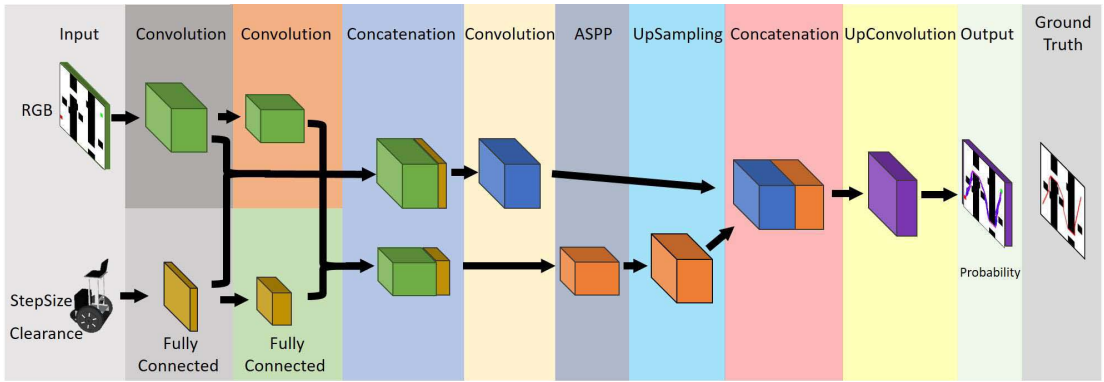
\includegraphics[width=\textwidth]{cnn_architecture}
\centering
\caption{Architecture of CNN model for NRRT*}
\label{fig:architecture}
\end{figure}

To generate the training data, start states and target states were randomly selected from a randomly selected subset of 5547 201 x 201 image dataset, resulting in 26960 combinations of start and target states with their corresponding optimal paths generated by running the A* algorithm. The optimal paths were converted to ground truth binary labels by assigning each pixel a value of 0 or 1, 0 for states not included in the optimal path, and 1 for pixels residing on the optimal path found by the A* algorithm. The same map image dataset was used for the simulations, refer to Section \ref{sec:dataset description} for additional details on the dataset. To train the CNN model, we assign individual pixels of the training images with pixel values from 0 to 3, where 0 represents a free state, 1 represents a state occupied by an obstacle, and 2 and 3 represent the start and target states respectively. The loss function is defined as:
\begin{align}
    L = \sum_{}^{} ce(\mathcal{O}, \mathcal{G})
\end{align}
where $\mathcal{O}$ is the output of the network, $\mathcal{G}$ is the ground truth label, and $L$ is the sum of cross-entropy loss across all training observations. As per the instructions of \cite{nrrt}, Adam optimizer with $\epsilon$ = 1e-4, $\beta_1$ = 0.9, and $\beta_2$ = 0.999 was used for the training process, while using a reduced batch size of 10 due to hardware limitations.
    
\subsection{Description of the Simulation Process}
\label{sec:description}
The dataset \cite{dataset} used for the simulation based evaluation of the three algorithms consists of 7 images from 7 distinct categories: alternating gaps, bugtrap forest, forest gaps and forest, mazes, single bugtraps, and multiple bugtraps. The images and their corresponding start/target state combinatinos is displayed in Figure \ref{fig:data}.

\begin{figure}[H]
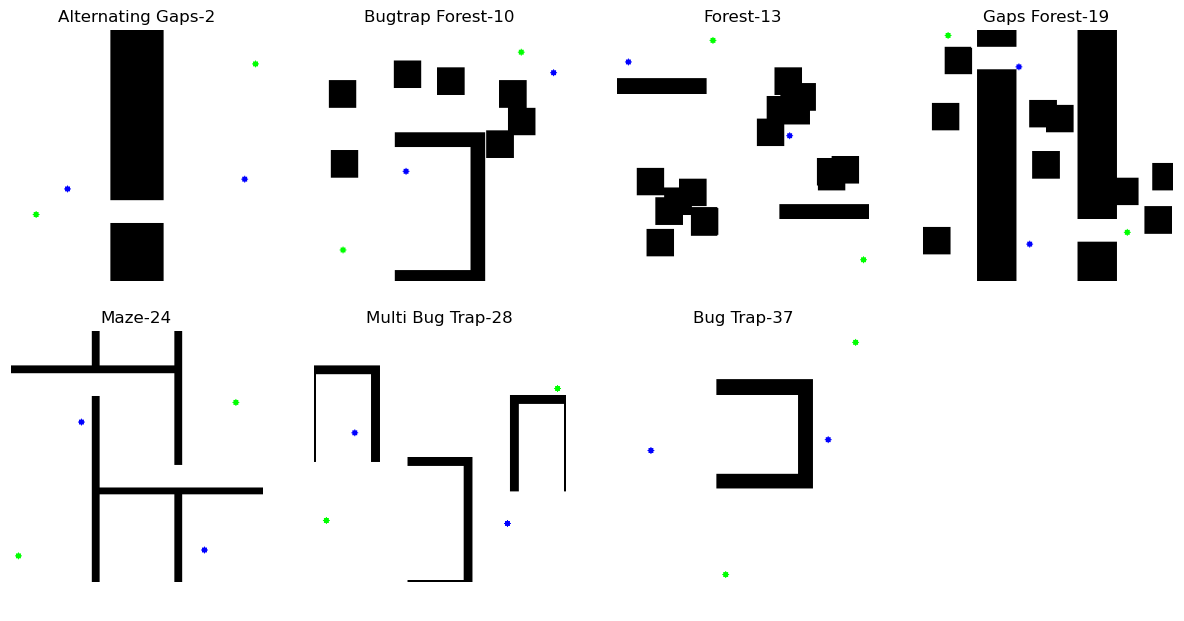
\includegraphics[width=\textwidth]{map_data}
\centering
\caption{Map images used for simulations, start/target states paired by same color}
\label{fig:data}
\end{figure}

All start/target pairs have a reachable path with the exception of one pair in \emph{Maze-24}, and most start/target pairs are blocked by one or more obstacles, and are not directly reachable. To observe the variation in execution time, calculated path cost, and success rate of the three algorithms in various scenarios with statistical significance, each algorithm will execute its path planning 5 times per state/target combination, for two state/target combinations on 7 maps, with 9 different batch sizes for sampling ([5, 10, 20, 40, 80, 100, 300, 600, 1000]), resulting in a total of 630 runs per each algorithm. The resulting metrics (further discussed in \ref{sec:Evaluation}) will be plotted grouped by map type and state/target pair to observe their respective patterns

 %===============================================================================

\section{Evaluation}
\label{sec:Evaluation}

This section is structured as follows: First, we mathematically define the different path-planning metrics used in the evaluation scheme. Then, we compare the performance of algorithms based on these metrics (using trend-plots generated from the simulations) to understand their behaviour in different situations. We describe a few, specific, state-space scenarios as well as some algorithmic factors and discuss their effects on the different metrics. Finally, we provide a qualitative comparison for the different paths generated by the algorithms for a specific subset of the maps and states.

\subsection{Defining the Metrics}

\subsubsection{Solution Cost ($\mathcal{J}$)}

The solution cost, $\mathcal{J}$, is defined as the cost-to-come to the goal location ({\varfont goal}) from the start location ({\varfont start}) along the path defined by the path-planning algorithm. We evaluate the cost ($\mathcal{J}$) as follows: For a set of N nodes in the free space $\mathcal{X}_{free}$, let $\mathcal{P} \subset \mathcal{X}_{free}$ be the set of nodes along the optimal path as computed by the path planning algorithm $\{ \mathcal{X}_{free}, x_{init}, \mathcal{G}(x_{goal})\}$; Then the cost $\mathcal{J}$ is defined as: 
\begin{align}
    \mathcal{J} = \sum_{i=1}^{N} ||x_i - Parent(x_i)||_2 \text{, where } x_i \in \mathcal{P}
\end{align}

\subsubsection{Execution Time ($\mathcal{T}$)}

We evaluate the execution time, $\mathcal{T}$,  as follows: Let, $\tau_{fmt}$, $\tau_{bit}$ and $\tau_{nrrt}$ denote the time-per-iteration for the FMT*, BIT* and NRRT* algorithms respectively. Let, $n_{fmt}$ and $n_{nrrt}$ denote the number of iterations performed by FMT* and NRRT*, respectively, before they find a solution. Also, we cap the maximum number of iterations that can be performed by each algorithm with a common value. Let this be $n\_max$. Then the execution time $\mathcal{T}$ is defined as:

\begin{align}
	\text{FMT*,} \quad \mathcal{T}_{fmt} &= \min(n_{fmt}, n\_max) \times \tau_{fmt} \\
	\text{NRRT*,} \quad \mathcal{T}_{nrrt} &= \min(n_{nrrt}, n\_max) \times \tau_{nrrt} \\
	\text{BIT*,} \quad \mathcal{T}_{bit} &= 
	\left\{
		\begin{array}{ll}
			\tau_{bit}  & \mbox{if } \mathcal{J}_{bit} = ||\text{\varfont start} - \text{\varfont goal}||_2\\
			n\_max \times \tau_{bit} & \mbox{otherwise} 
		\end{array}
	\right.
\end{align}

Due to the anytime resolution of BIT*, its execution time is recorded differently then FMT* and NRRT*. For FMT* and NRRT*, the final execution time it takes for the algorithm to find any feasible solution from {\varfont start} to {\varfont goal} is recorded. For BIT*, the execution time is recorded on each iteration of the algorithm.

\subsubsection{Success Rate ($\mathcal{Q}$)}

For sampling based algorithms, the random sampling of potential nodes in the graph/tree introduces an additional "uncertainty" (alongwith the feasibility) in the ability of the algorithm to find any feasible solution. This uncertainty can be modeled as the entropy precipitating from the probabilistic distribution used for the random-sampling.

Therefore, it is important to quantify the tolerance of an algorithm to this uncertainty. We achieve this by computing the success rate for each algorithm over $N$ runs - on the same map with the same {\varfont start} and {\varfont goal} states - using a different seed values for the random-generator function in each run. The success rate, for a specific map with fixed {\varfont start} and {\varfont goal} states, is defined as:

\begin{align}
    \mathcal{Q} = \frac{\sum_{i=1}^{N} \mathbbm{1}(\text{\varfont hasPath[start, goal]} = True)}{N}
\end{align}

where, {\varfont hasPath[start, goal]} returns $True$ if the algorithm is able to find a path from {\varfont start} to {\varfont goal}. We have used $N=5$ for our simulations.


\subsubsection{Sample Count ($\mathcal{N}$)}

Sample count is defined differently for FMT* and BIT*/NRRT*. For FMT*, the sample count is fixed before the algorithm begins finding a path. However, both BIT* and NRRT* perform sampling in batches. Therefore, the final sample count for BIT* and NRRT* depends on the number of iterations the algorithm performs.

For, FMT*, we have used the following sample counts: $[5, 10, 20, 40, 80, 100, 300, 600, 1000]$. NRRT* used the same range of sample counts as batch sizes, meaning that as the batch size increases, there are less opportunities to switch between the uniform and non-uniform sampling methods, and initial call to \emph{Rand()} can significantly impact the outcome of the planner as the batch size increases. For BIT*, a cumulative value of the number of points sampled in each batch is recorded.

\subsubsection{Number of collision checks ($\mathcal{C}$)}
This is defined as the total number of calls each algorithm makes to {\varfont CheckCollision} before adding a node to the graph/tree. (Refer each algorithm's methodology for performing the collision check as defined in \ref{sec:Methodology})

\subsection{Performance Analysis: Metric evaluation}

\subsubsection{Solution Cost ($\mathcal{J}$) vs Execution Time ($\mathcal{T}$) (refer Fig. \ref{met:scVet})}

\begin{figure}
	\makebox[\linewidth]{
		\begin{tabular}{cc}
			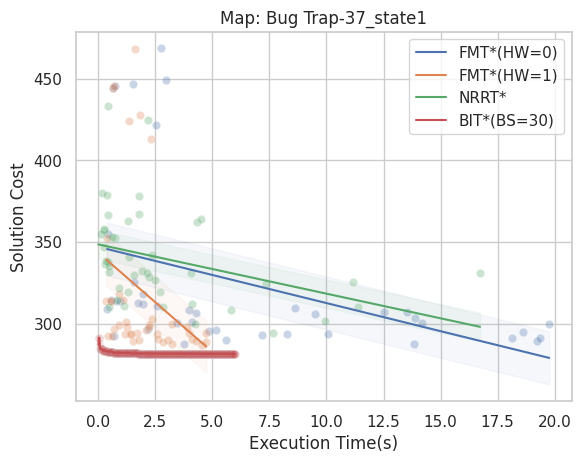
\includegraphics[scale=0.45]{scVet_Bug Trap-37_state1.png} & 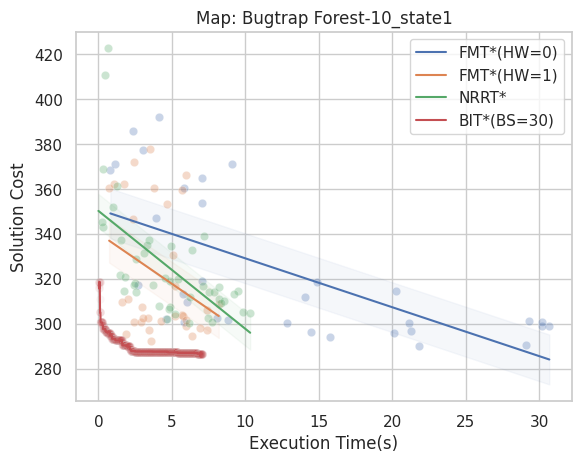
\includegraphics[scale=0.45]{scVet_Bugtrap Forest-10_state1.png}  \\
			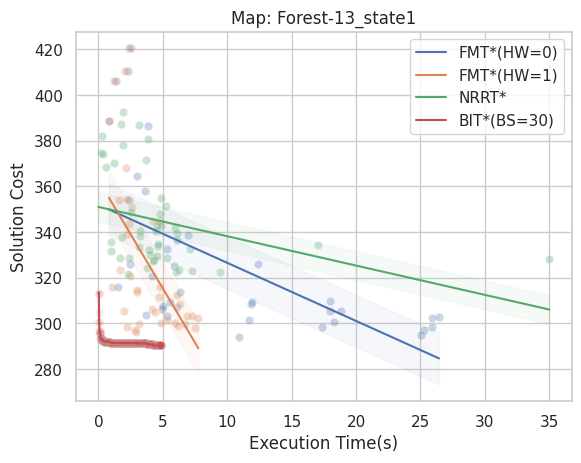
\includegraphics[scale=0.45]{scVet_Forest-13_state1.png} & 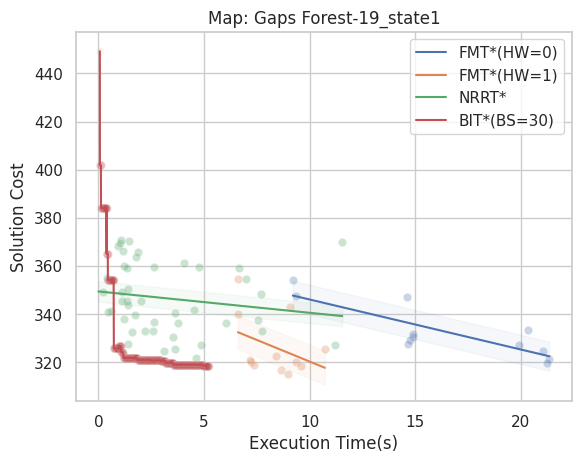
\includegraphics[scale=0.45]{scVet_Gaps Forest-19_state1.png}    \\
			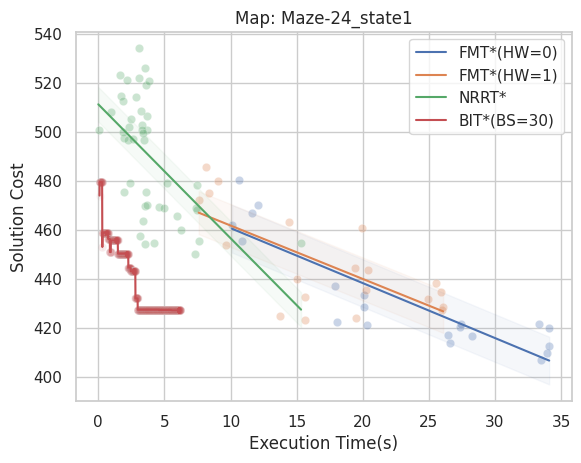
\includegraphics[scale=0.45]{scVet_Maze-24_state1.png} & 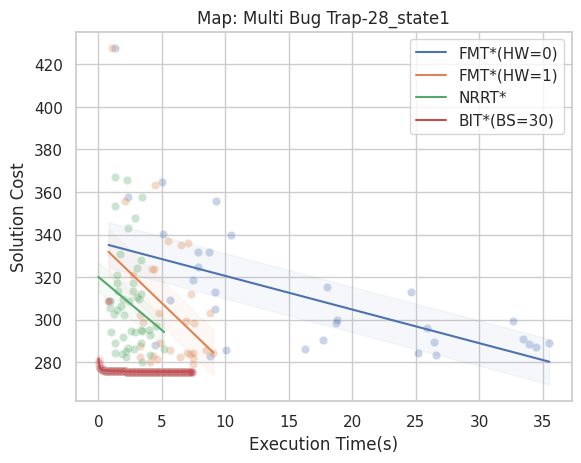
\includegraphics[scale=0.45]{scVet_Multi Bug Trap-28_state1.png}  \\
		\end{tabular}
	}
	\caption{Comparing solution cost with runtime for FMT* without heuristics (blue), FMT* with euclidean-heuristics (weigth=1.0) (orange), BIT* with batch-size=30 (red) and NRRT* (green) in different map environments}
        \label{met:scVet}
\end{figure}

BIT* shows the best performance in most cases with a faster convergence rate to a more optimal solution as it achieves the lowest solution cost in most cases. It is also observed that in some cases the solution cost for BIT* remains constant over a certain number of iterations but drops to a lower solution cost with sufficiently large number of iterations. 

FMT* with euclidean-heuristics always performs much better than the standard FMT* as expected. FMT* with heuristics also seems to perform better than NRRT* in most cases. Generally, the solution cost decreases with increasing execution time.

\subsubsection{Success Rate ($\mathcal{Q}$) vs Execution Time ($\mathcal{T}$) (refer Fig. \ref{met:srVet})}

\begin{figure}
	\makebox[\linewidth]{
		\begin{tabular}{cc}
			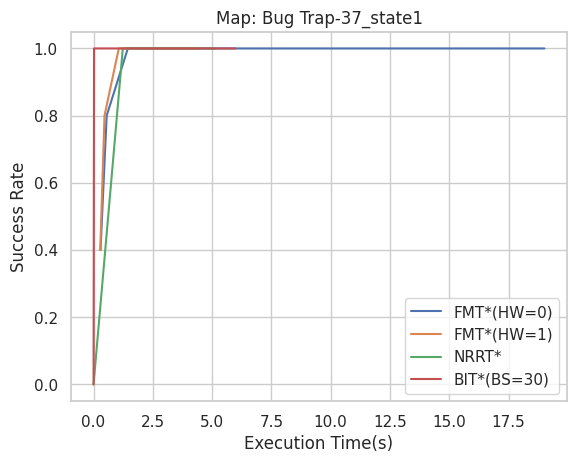
\includegraphics[scale=0.45]{srVet_Bug Trap-37_state1.png} & 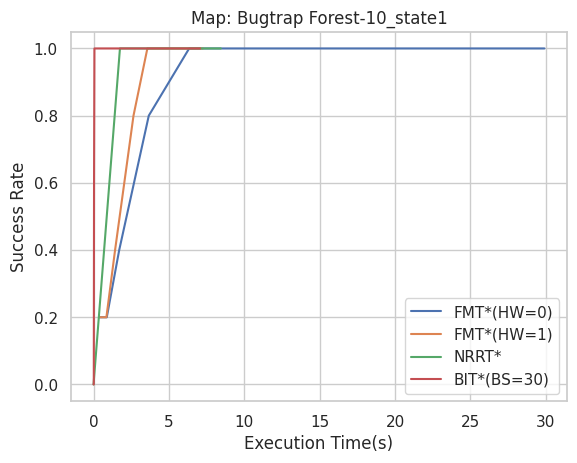
\includegraphics[scale=0.45]{srVet_Bugtrap Forest-10_state1.png}  \\
			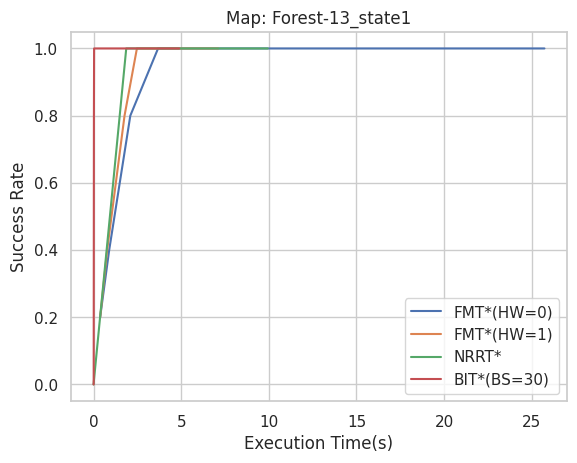
\includegraphics[scale=0.45]{srVet_Forest-13_state1.png} & 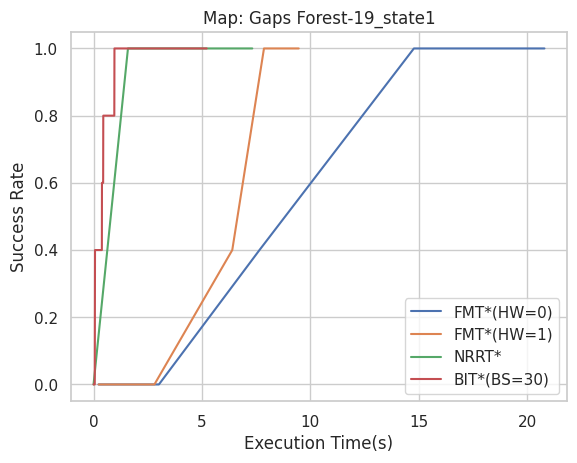
\includegraphics[scale=0.45]{srVet_Gaps Forest-19_state1.png}    \\
			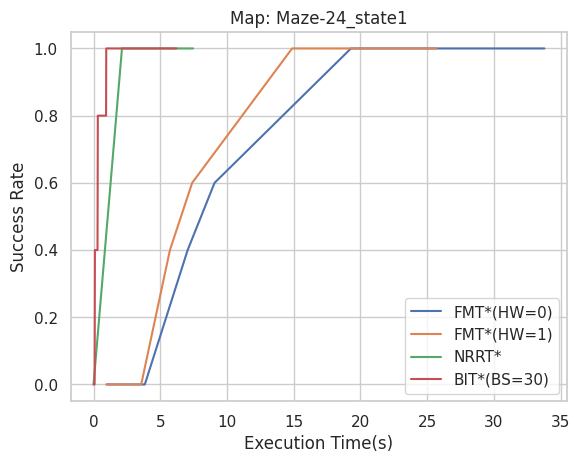
\includegraphics[scale=0.45]{srVet_Maze-24_state1.png} & 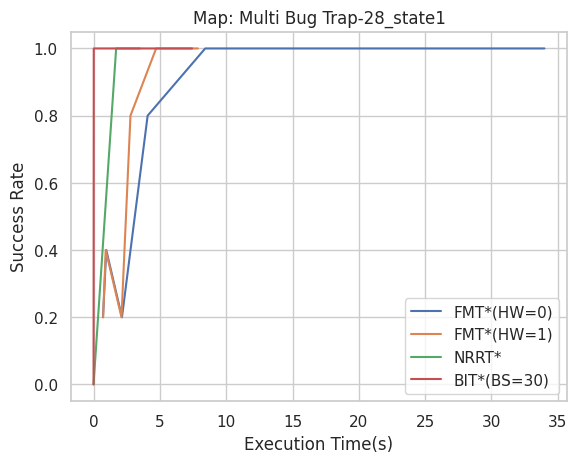
\includegraphics[scale=0.45]{srVet_Multi Bug Trap-28_state1.png}  \\
		\end{tabular}
	}
	\caption{Comparing success rate with runtime for FMT* without heuristics (blue), FMT* with euclidean-heuristics (weigth=1.0) (orange), BIT* with batch-size=30 (red) and NRRT* (green) in different map environments}
        \label{met:srVet}
\end{figure}

All algorithms reach $\mathcal{Q}=1.0 (\hat{\mathcal{Q}})$ within 5 seconds of execution for almost all the map environments. Only in the case of Maze and Gaps Forest, FMT* takes much longer to achieve $\hat{\mathcal{Q}}$. BIT* is the fastest in achieving $\hat{\mathcal{Q}}$ with the other algorithms showing only a marginally slower convergence in most map environments. FMT* without heuristcs is the slowest to converge in all scenarios

\subsubsection{Success Rate ($\mathcal{Q}$) vs Sample Count 
\label{sec:sucess_rate}
($\mathcal{N}$) (refer Fig. \ref{mets:srVsc})}

\begin{figure}
	\makebox[\linewidth]{
		\begin{tabular}{cc}
			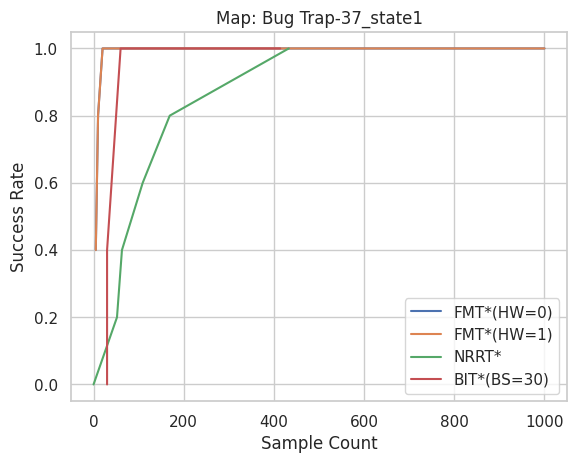
\includegraphics[scale=0.45]{srVsc_Bug Trap-37_state1.png} & 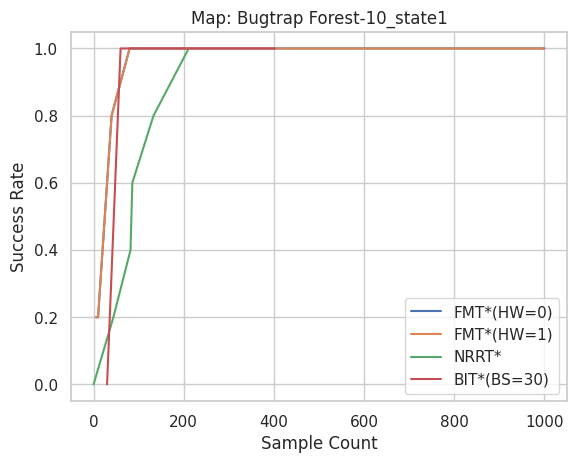
\includegraphics[scale=0.45]{srVsc_Bugtrap Forest-10_state1.png}  \\
			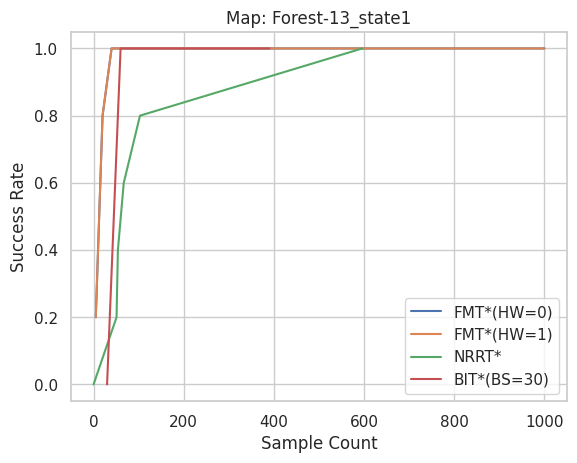
\includegraphics[scale=0.45]{srVsc_Forest-13_state1.png} & 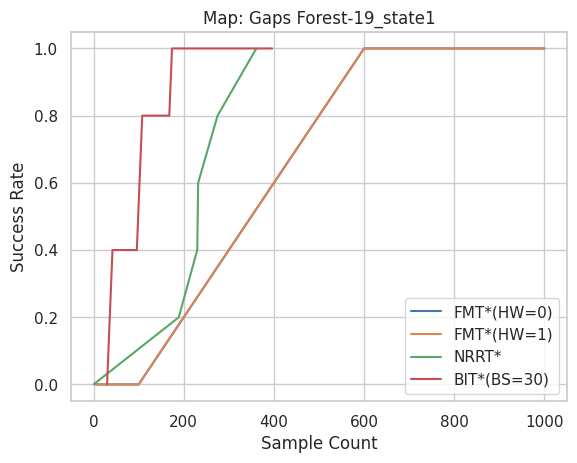
\includegraphics[scale=0.45]{srVsc_Gaps Forest-19_state1.png}    \\
			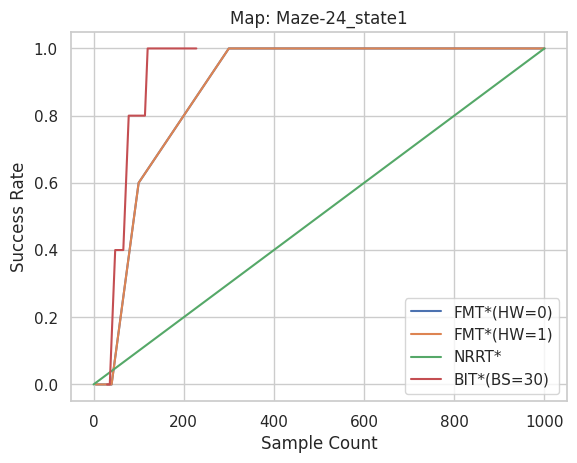
\includegraphics[scale=0.45]{srVsc_Maze-24_state1.png} & 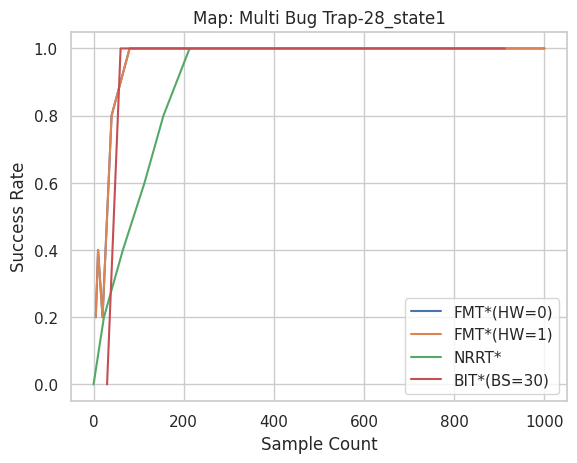
\includegraphics[scale=0.45]{srVsc_Multi Bug Trap-28_state1.png}  \\
		\end{tabular}
	}
	\caption{Comparing success rate with sample count for FMT* without heuristics (blue), FMT* with euclidean-heuristics (weigth=1.0) (orange), BIT* with batch-size=30 (red) and NRRT* (green) in different map environments}
        \label{mets:srVsc}
\end{figure}

For BugTrap and Forest (simple environments), FMT* requires a relatively smaller sample count ($\sim 80$) to achieve $\hat{\mathcal{Q}}$. However, for more complex enviroments such as BugTrap-Forest, Gaps-Forest, Maze and Multi-BugTrap, BIT* achieves $\hat{\mathcal{Q}}$ most efficiently. 

A noteworthy point about BIT* is that it is able to achieve $\hat{\mathcal{Q}}$ with almost the same sample count ($\sim 100$) in all map environments. NRRT* seems to require a relatively larger sample count to achieve $\hat{\mathcal{Q}}$ in most map environments.

\subsubsection{Sample Count ($\mathcal{N}$) vs Number of collision checks ($\mathcal{C}$) (refer Fig. \ref{mets:scVcc})}

\begin{figure}
	\makebox[\linewidth]{
		\begin{tabular}{cc}
			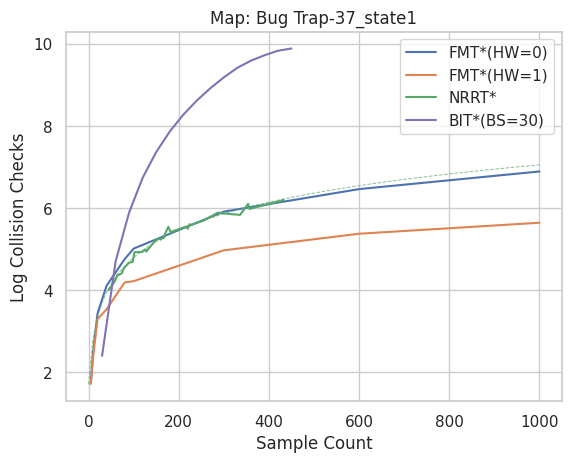
\includegraphics[scale=0.45]{scVcc_Bug Trap-37_state1.png} & 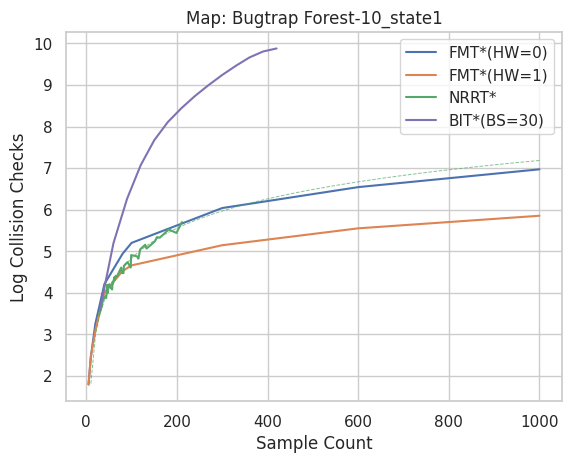
\includegraphics[scale=0.45]{scVcc_Bugtrap Forest-10_state1.png}  \\
			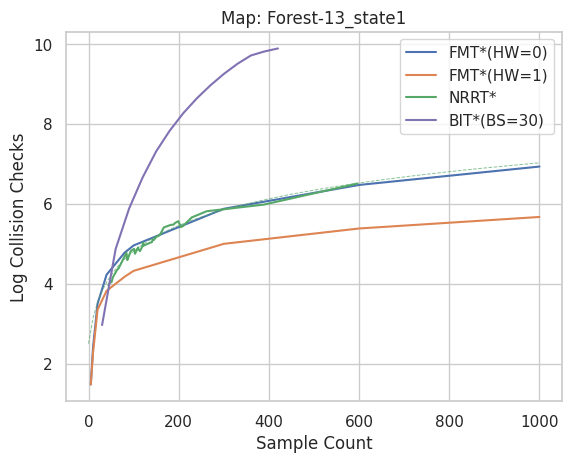
\includegraphics[scale=0.45]{scVcc_Forest-13_state1.png} & 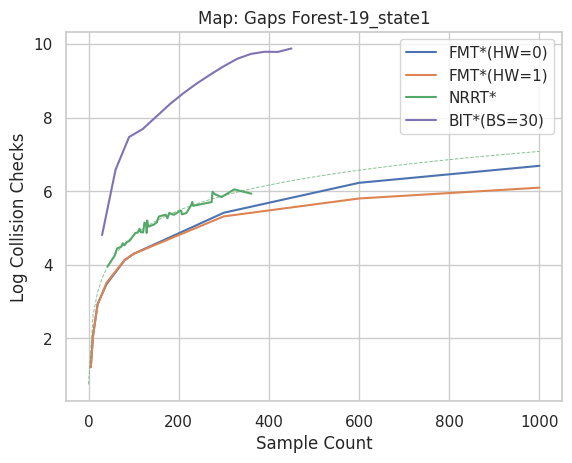
\includegraphics[scale=0.45]{scVcc_Gaps Forest-19_state1.png}    \\
			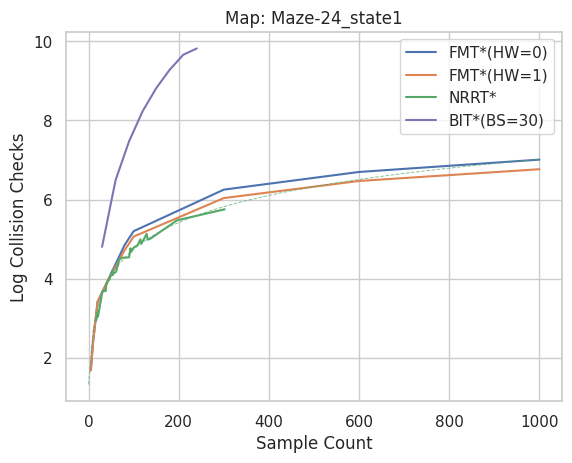
\includegraphics[scale=0.45]{scVcc_Maze-24_state1.png} & 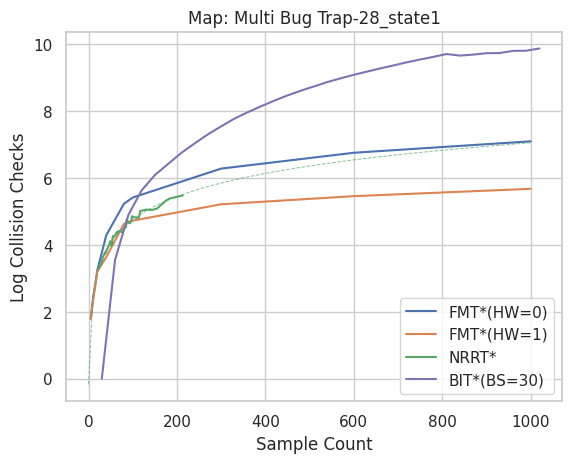
\includegraphics[scale=0.45]{scVcc_Multi Bug Trap-28_state1.png}  \\
		\end{tabular}
	}
	\caption{Comparing sample count with number of collision checks made by FMT* without heuristics (blue), FMT* with euclidean-heuristics (weigth=1.0) (orange), BIT* with batch-size=30 (red) and NRRT* (green) in different map environments}
        \label{mets:scVcc}
\end{figure}

In this analysis, it is clearly observed that FMT* performs significantly fewer collision checks compared to BIT*. FMT* with euclidean-heuristics performs the least number of collision checks. FMT* performs the maximum number of collision checks for the maze environment. The significantly lower number of collision checks for FMT* is due to its "lazy collision checking" behavior which is what makes it perform better in high dimensional environments. 

\subsection{Qualitative Analysis: Generated Paths}

\textbf{\underline{FMT*:}}

FMT* progressively improves on the optimality of the path found as the sample count is increased. This can be observed from the paths generated by FMT* for the Maze environment with increasing sample count as shown in Fig. \ref{fmt:nsamples}

\begin{figure}
	\makebox[\linewidth]{
		\begin{tabular}{ccc}
			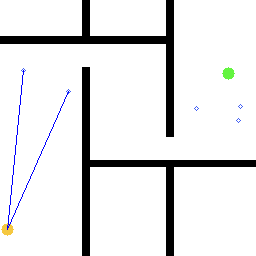
\includegraphics[scale=0.45]{fmt_paths/n_samples/0.png} & 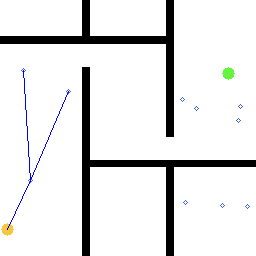
\includegraphics[scale=0.45]{fmt_paths/n_samples/1.png} & 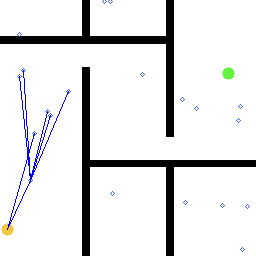
\includegraphics[scale=0.45]{fmt_paths/n_samples/2.png}\\
			(a) & (b) & (c)\\[6pt]
			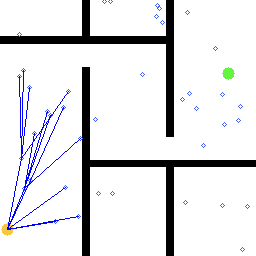
\includegraphics[scale=0.45]{fmt_paths/n_samples/3.png} & 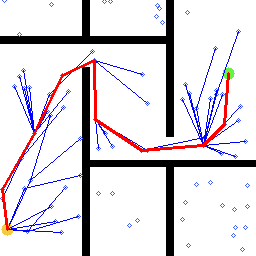
\includegraphics[scale=0.45]{fmt_paths/n_samples/4.png} & 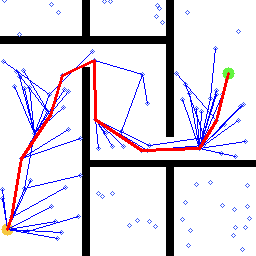
\includegraphics[scale=0.45]{fmt_paths/n_samples/5.png}\\
			(d) & (e) & (f)\\[6pt]
			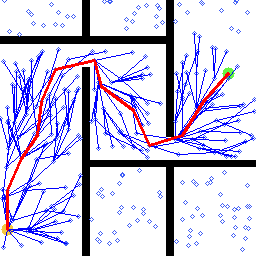
\includegraphics[scale=0.45]{fmt_paths/n_samples/6.png} & 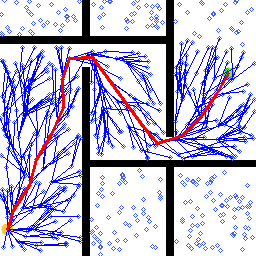
\includegraphics[scale=0.45]{fmt_paths/n_samples/7.png} & 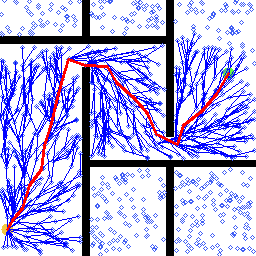
\includegraphics[scale=0.45]{fmt_paths/n_samples/8.png}\\
			(g) & (h) & (i)\\[6pt]
		\end{tabular}
	}
	\caption{Paths generated by FMT* (without heuristics) for the maze environment with increasing sample count: (a)-5, (b)-10, (c)-20, (d)-40, (e)-80, (f)-100, (g)-300, (h)-600, (i)-1000. Red line indicates the final path generated by the algorithm}
	\label{fmt:nsamples}
\end{figure}

As the sample count increases, the algorithm is able to avoid unnecessary turns to generate a path with longer linear-subpaths thus minimizing the cost.

An additional set of simulations were performed for FMT* specifically which incorporates euclidean-heuristics (as described in \ref{met:fmt}). The paths generated by each FMT* algorithm on the Forest map is described in Fig \ref{fmt:heur}.

\begin{figure}[H]
	\makebox[\linewidth]{
		\begin{tabular}{cc}
			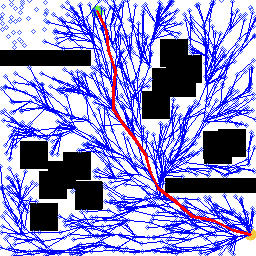
\includegraphics[scale=0.45]{fmt_paths/heuristics/0.png} & 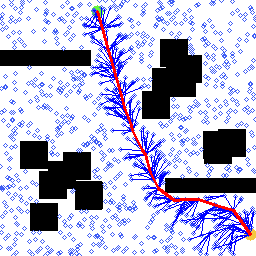
\includegraphics[scale=0.45]{fmt_paths/heuristics/1.png} \\
			(a) & (b)\\[6pt]
		\end{tabular}
	}
	\caption{Paths generated by FMT* on the Forest map: (a)- without heuristics and (b) - with euclidean-heuristics (weight=1.0). Red line indicates the final path generated by the algorithm. Blue lines indicate the nodes visited by the algorithm}
	\label{fmt:heur}
\end{figure}

FMT* with euclidean-heuristics visits fewer nodes while searching for a path and is thus able to converge faster. Since we use euclidean-heuristics with a euclidean cost-to-come to pick the next node in the tree, FMT* with heuristics is able to generate a more optimal path than the standard FMT* algorithm.

\textbf{\underline{BIT*:}}

The final paths produced by BIT* were mostly identical, with only a few minor differences. The reason for the similarity is that the maximum number of iterations was set to a large value, allowing all runs to converge closer to the optimal path. Still, the differences were more noticeable for more complicated environments. Figure \ref{bit:finalpaths} shows a highlight of some of the paths produced by the algorithm. In case of the existence of the minor differences, the better paths have been selected. These images show some of the characteristics of BIT*. For example, they show a higher sampling density in some regions. That is because BIT* samples in the region that contains a more optimal path than the current solution. This is most obvious in Fig \ref{bit:finalpaths} (g). However, it seems to be an ineffective strategy for the maze in Fig \ref{bit:finalpaths} (e). The images also show that the spanning tree in BIT* is constructed starting from the {\varfont start} state, as seen from the density of the blue lines. Finally, the images demonstrate the ability of BIT* to find a path through relatively narrow openings, as seen best in Fig \ref{bit:finalpaths} (d).

\begin{figure}
	\makebox[\linewidth]{
		\begin{tabular}{ccc}
			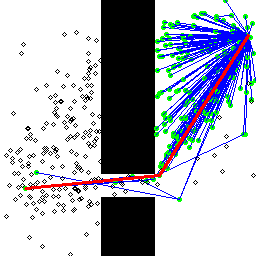
\includegraphics[scale=0.45]{imgs/bit_paths/one_per_map/bitstar_result_20154.png} & 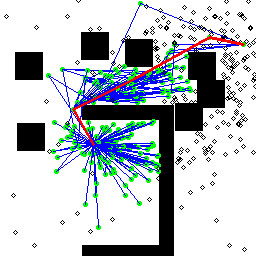
\includegraphics[scale=0.45]{imgs/bit_paths/one_per_map/bitstar_result_20903.png} & 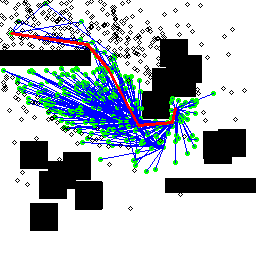
\includegraphics[scale=0.45]{imgs/bit_paths/one_per_map/bitstar_result_21200.png}\\
			(a) & (b) & (c)\\[6pt]
			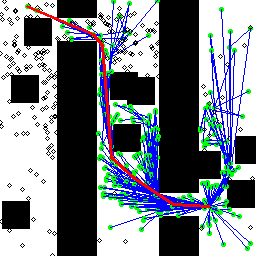
\includegraphics[scale=0.45]{imgs/bit_paths/one_per_map/bitstar_result_21852.png} & 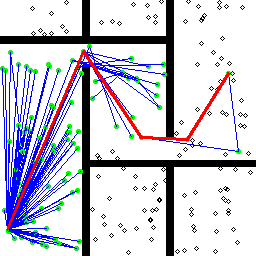
\includegraphics[scale=0.45]{imgs/bit_paths/one_per_map/bitstar_result_22351.png} & 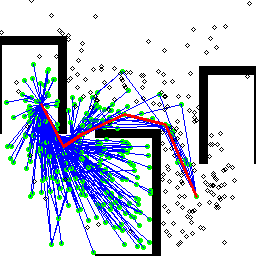
\includegraphics[scale=0.45]{imgs/bit_paths/one_per_map/bitstar_result_22704.png}\\
			(d) & (e) & (f)\\[6pt]
			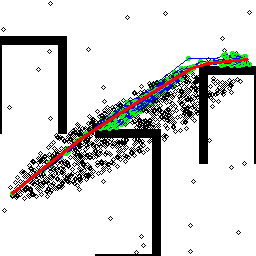
\includegraphics[scale=0.45]{imgs/bit_paths/one_per_map/bitstar_result_22754.png} & 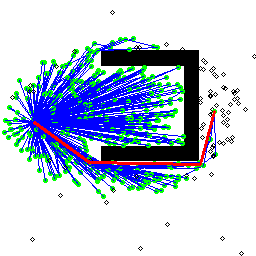
\includegraphics[scale=0.45]{imgs/bit_paths/one_per_map/bitstar_result_23604.png} & 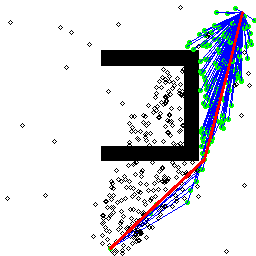
\includegraphics[scale=0.45]{imgs/bit_paths/one_per_map/bitstar_result_23653.png}\\
			(g) & (h) & (i)\\[6pt]
		\end{tabular}
	}
	\caption{Paths generated by BIT* (Batch Size=30) for various maze environments. Red line indicates the final path generated by the algorithm}
	\label{bit:finalpaths}
\end{figure} 

\textbf{\underline{NRRT*:}}\\
It is evident from the generated paths, distribution of the non-uniform sampling space, and the nodes explored in \ref{fig:nrrt} that the CNN did not adequately estimate the probability distribution corresponding to optimal paths generated by the A* algorithm.

\begin{figure}
\centering
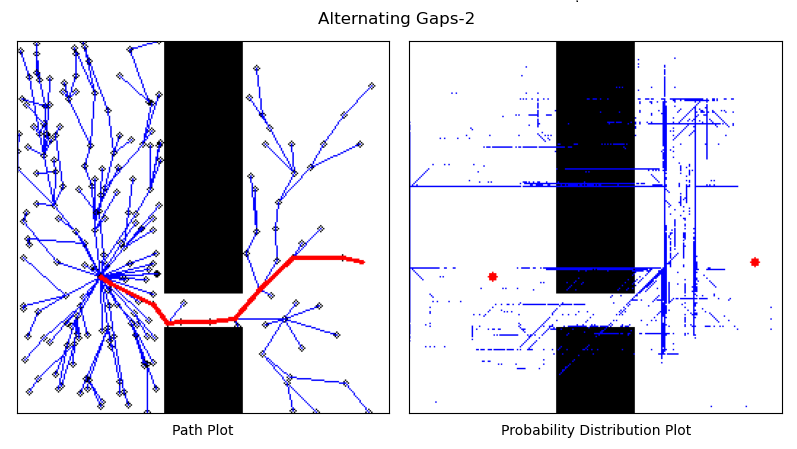
\includegraphics[scale=0.5]{nrrt_plot}
\caption{Path plot and sampling distribution plot of Alternating Gaps-2; Red indicates start/target states + computed path, blue indicates $p(optimal) > 0.5$ in the distribution plot}
\label{fig:nrrt}
\end{figure}

It can be seen from visual inspection of Figure \ref{fig:nrrt} that the computed path is sub-optimal. The explored nodes and their corresponding paths are extending outwards in a straight manner, similar to the paths generated from RRT* due to the rewiring procedure. The fact that the plot paths closely resembles paths generated from RRT* is an indication that even with the sampling rate $\alpha = 0.5$, the non-uniform sampling is not contributing much in the exploration of the state space. When observing the distribution plot, it is evident that pixels with high probabilities of being on the optimal path do not correspond to the pixels associated with the actual optimal path. Furthermore, a non-negligible amount of the pixels identified as optimal lie on obstacles, meaning sampling from these regions will increment the algorithm iterations and collision check count with no improvements to the path planning task. We can observe the probability distribution learned on each of the images for a single state in Figure \ref{fig:all_prob}.

\begin{figure}
\centering
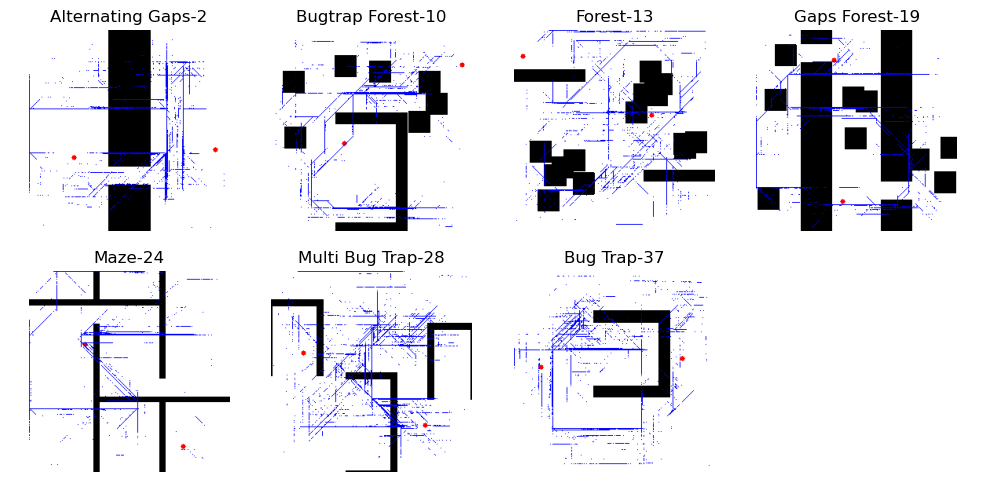
\includegraphics[scale=0.6]{all_prob}
\caption{Probability distribution of pixel being on an optimal path; Red indicates start/target states + computed path, blue indicates $p(optimal) > 0.5$}
\label{fig:all_prob}
\end{figure}

It is also evident from the distribution plots that the model did not converge to a state that can adequately bias the sampling process towards an optimal path. However, it can be seen that the probability distributions follow some structured combination of straight line paths and paths angled off at 45$\degree$ angles. It may be the case that further training with additional data may lead to the increase in model performances in terms of the accuracy of the probability distribution approximation. Refer to Figure \ref{fig:nrrt_ideal} for the probability distribution generated by NRRT* with the CNN model working as intended.

\begin{figure}
\centering
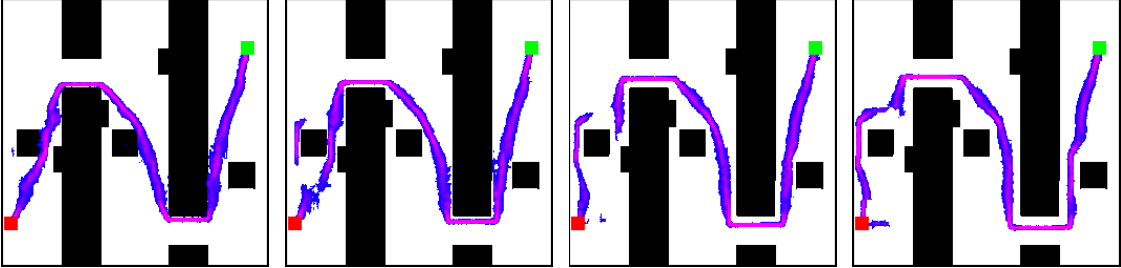
\includegraphics[scale=0.5]{nrrt_ideal}
\caption{Reported probability distributions of NRRT* by the original authors \cite{nrrt}}
\label{fig:nrrt_ideal}
\end{figure}

In the ideal case, non-uniform sampling state should have polarized probabilities, with a near-continuous path of pixels with high probabilities from the start state to the target state. Compared to other sampling-based methods, this would significantly reduce the number of iterations required for convergence, while maintaining near-optimal path costs even for environments with higher dimensions (given that the CNN has been adequately trained). Further discussions on the limitations of the CNN model performance can be found in Section \ref{sec:cnn_failure}.

It is evident from Figure \ref{met:scVet} that the implemented NRRT* algorithm performs nearly as well as FMT*, but performs inferior to BIT* and FMT* with euclidean heuristics both in terms of execution time and path costs. As discussed in Section \ref{sec:sucess_rate}, NRRT* is among the algorithms that achieve $\hat{\mathcal{Q}}$ faster then FMT* instanaces. However, it is displayed in Figure \label{met:srVet} that more samples are required for NRRT* to achieve $\hat{\mathcal{Q}}$. This is an indication that on average, NRRT* takes less computation time per iteration. It is also an indication that the other algorithms are able to achieve more with a smaller sample of states. From Figure \ref{mets:scVcc}, it can be seen that sample count has a linear relationship with collision checks (i.e. logarithmic relationship in log space). This behaviour is to be expected since NRRT* does not make improvements on reducing the number of collision checks with respect to each iteration. 

\subsection{Analyzing edge-cases: State Specific Configurations}

\subsubsection{Straight line paths}
\label{sec:straight_line}
In one of the simulations run on the Gaps-Forest map, the path from {\varfont start} to {\varfont goal} was a straight line with no obstacles along this line. In this section, we qualitatively compare the paths generated by each algorithm in such a scenario
\pagebreak

\textbf{\underline{FMT*:}}

\begin{figure}[H]
	\makebox[\linewidth]{
		\begin{tabular}{cc}
			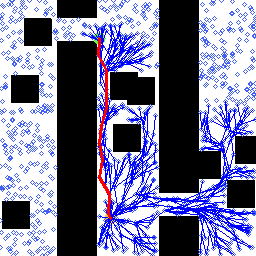
\includegraphics[scale=0.4]{fmt_paths/straight_line/0.png} & \includegraphics[scale=0.4]{fmt_paths/straight_line/1.png} \\
			(a) & (b)\\[6pt]
		\end{tabular}
	}
	\caption{Paths generated by FMT* on the Gaps-Forest map: (a)- without heuristics and (b) - with euclidean-heuristics (weight=1.0). Red line indicates the final path generated by the algorithm. Blue lines indicate the nodes visited by the algorithm}
	\label{fmt:straightlinepath}
\end{figure}

Even with a 1000 sample count, FMT* is unable to find the straight-line path. FMT* with euclidean-heuristics is closer to the straight-line path. If the number of samples is increased, FMT* will be able to find the straight line path

\textbf{\underline{BIT*:}}

\begin{figure}[H]
	\makebox[\linewidth]{
		\begin{tabular}{c}
			\includegraphics[scale=0.4]{bit_paths/straight_line/0.png} \\
		\end{tabular}
	}
	\caption{Path generated by BIT* on the Gaps-Forest map. Red line indicates the final path generated by the algorithm.}
	\label{bit:straightlinepath}
\end{figure}

BIT* takes only a single iteration of a fixed batch-size to find the straight-line path. Therefore, in this specific case, BIT* will always outperform its counterparts both in terms of optimality as well as computational complexity

\textbf{\underline{NRRT*:}}

\begin{figure}[H]
	\makebox[\linewidth]{
		\begin{tabular}{c}
			\includegraphics[scale=0.4]{nrrt_paths/straight_line/0.png} \\
		\end{tabular}
	}
	\caption{Path generated by NRRT* on the Gaps-Forest map. Red line indicates the final path generated by the algorithm.}
	\label{nrrt:straightlinepath}
\end{figure}

NRRT* also struggles to find and the optimal straight-line path. In theory, if the CNN accurately estimates the optimal pixel probabilities, NRRT* should be able to compute a path with less deviations away from the straight line. This is especially true if the steering radius was reduced. The path cost would increase at the cost of additional execution time.

\subsubsection{Unreachable goals}

Often times, there are cases where the goal is unreachable from the start location on the map. We outline one such case that we encountered during our simulations for the Maze environment where the goal was entirely enclosed by obstacles. In such situations, it is important to evaluate how fast can the algorithm can report "no-solution". This can be evaluated using two metrics: Mean execution time per sample count and Mean number of collision check per sample count. We compute and report these metrics for the three algorithms in Table. \ref{un:mets}.

\begin{table}[H]
	\caption{Running FMT*, BIT* and NRRT* on a map with an unreachable goal}
	\makebox[\linewidth]{
		\begin{tabular}{|c|c|c|}
			\hline
			Alg. & \begin{tabular}{@{}c@{}}Mean execution time \\ per sample count\end{tabular} & \begin{tabular}{@{}c@{}}Mean no. collision checks \\ per sample count\end{tabular}\\
			\hline
			FMT* & 0.082 & 1.48\\
			\hline
			\begin{tabular}{@{}c@{}}FMT* \\ (with heuristics)\end{tabular} & 0.080 & 1.48\\
			\hline
			BIT* & 0.021 & 63.25\\
			\hline
			NRRT* & 0.026 & 1.19\\
			\hline
		\end{tabular}
		}
	\label{un:mets}
\end{table}

\section{Limitations}

Our comparative study shows limitations in each of the three sampling based algorithms. As seen in Fig \ref{met:scVet}, FMT* and NRRT* had very long execution times even on low Sample Counts. Such times are impractical for real world path planning applications. On the other hand, as seen in Fig \ref{mets:scVcc}, BIT* showed a nonlinear increase in the number of collision checks as the sample count is increased. This is problematic for applications that may require a greater number of sample counts, particularly high dimensional applications. Additionally, unlike FMT* and NRRT*, BIT* does not have a maximum steering distance. However, this means that it requires a larger number of checks for obstacles in each collision check. Therefore, with a greater number of more expensive collision checks, the performance of BIT* on higher dimensions may degrade significantly. However, due to limited time, we only evaluated the algorithms on the two dimensional case. Section \ref{sec:cnn_failure} describes a limitation we observed for NRRT* in detail and Section \ref{sec:future_work} proposes some opportunities for future work.

\subsection{NRRT* CNN}
\label{sec:cnn_failure}
As discussed earlier in Section \ref{sec:straight_line}, it was evident that the non-uniform sampling did not contribute much towards biasing the non-uniform sampling distribution towards that of an optimal distribution. There are no indications of obvious issues from the training convergence plot as shown in Figure \ref{fig:convergence}. It is evident from the convergence plot that the training process is quite stable, and both the training and testing losses converge to a stable minimum. There are multiple factors that may have contributed to the sub-optimal performance of the CNN model. The first reason being is that the original paper \cite{nrrt} does not disclose certain aspects of the CNN architecture (i.e. architecture for the decoding portion of the model, dilation values for atrous convolution, etc.) and contains some minor discrepancies in the description of the architecture (mismatching feature map size for listed dimension vs dimension calculated when steps are followed, illustration of CNN architecture and description mismatching, etc.). Although the general idea of the proposed CNN architecture was captured, the details of the implementation likely contain discrepencies from the original implementation. In addition, a Major difference between the CNN model from the original authors of NRRT* and the implemented model is that the size of the training dataset was much larger for the original authors. Optimal paths computed from the A* algorithm for ~1 million start/taget state combinations were generated between 5574 available images in the dataset \cite{dataset}. Due to time and compute resource limitations, the implemented model was only trained on 26960 observations, with nearly a 40-fold different in training data size for the CNN model of near identical complexity.

\begin{figure}[H]
\includegraphics[width=0.6\textwidth]{model_convergence}
\centering
\caption{Convergence of the CNN model during training}
\label{fig:convergence}
\end{figure}

\subsection{Recommendations for Future Work}
\label{sec:future_work}
To extend this work, further evaluation can be done by evaluating the Solution Cost against the Sample Count as well as the Collision Checks. This may help reveal additional information for the sampling efficiency and scalability of the three algorithms to higher dimensions. However, for the best evaluation of higher dimensional performance, it is recommended that the simulations be extended to higher dimensional tasks.

Furthermore, it is recommended that BIT* should be evaluated with a variable batch size as it may optimize the algorithm and help overcome plateaus. While a variation of this problem was implemented, it was not extensively evaluated in our project. Additionally, as observed in Fig \ref{bit:finalpaths} (h), BIT* focuses much of its optimization efforts closer to the {\varfont start} state. Adding a second spanning tree from the goal state, as in RRT-connect \cite{RRTConnect} may therefore help increase the convergence rate on complicated environments with many obstacles by allowing more optimization opportunities to be discovered more quickly.

With significant additional training data prepared, the CNN model for the NRRT* algorithm can be adequately trained to verity the reported performances. With a model that generalizes well, evaluations can be done for varying image resolutions, robot step sizes, and obstacle clearances to fully understand its performance.

By evaluating some of the strengths and weaknesses of FMT*, BIT*, and NRRT*, our comparative study also provides inspiration to combine various aspects of the algorithms to utilize their strengths. For instance, we may use a CNN model to perform non-uniform sampling in BIT* before a solution is found, and then use the current method of better possible solution to do sampling. We also recommend integrating the collision checking algorithm used by FMT* in BIT* to reduce the number of collision checks while maintaining anytime resolution, lower solution costs, and lower execution times.

\section{Conclusion}
In this report, we presented a quantitative and qualitative comparison of Fast Marching Trees (FMT*), Batch Informed Trees (BIT*), and Neural Rapidly-exploring Random Trees (NRRT*). These are three sampling based planning algorithms that aim to find the best path from a start point to a goal point efficiently. In our evaluation of these planners on various 2D maps, BIT* outperforms FMT* and NRRT* in the execution time, success rate, and solution cost. The solution cost and success rate of FMT* and NRRT* improves as the sample count is increased. However, a higher sample count results in a higher execution time. FMT* with heuristics outperforms FMT* without heuristics on all metrics. Additionally, FMT* (with and without heuristics) requires the fewest collision checks as the sample count is increased, which is a sign of better scalability for high dimensional tasks.

\subsection*{Acknowledgements}
Parts of the implemented algorithms incrementally modified some parts of the starter code provided in \href{https://github.com/florianshkurti/csc477_fall22/blob/master/path_planning_and_control_assignment/description/CSC477_Assignment_2.pdf}{CSC2630 Assignment 2}.

    
\clearpage

\bibliography{report}

\clearpage

\section*{Appendix A: Group Contributions}
\label{sec:AppendixA}
    
    Jazib Ahmad contributed towards the implementation of the BIT* planner and data collection. He also contributed to the development of the data generation and evaluation scheme and the development of configurable experiments.

    Jimmy Woo contributed towards the data collection, implementation and training of the CNN model, as well as the implementation of the NRRT* planner. He also contributed to the plot generation process.

    Sumant Bagri contributed towards implementing the original FMT* planner and its variant with heuristics. He was also responsible for defining and documenting the evaluation scheme as well as creating the pipeline for generating the evaluation metrics. 

\clearpage

\end{document}

%===============================================================================

% The maximum paper length is 8 pages excluding references and acknowledgements, and 10 pages including references and acknowledgements

%===============================================================================